\section{User Interface Elements} % (fold)
\label{sec:user_interface_elements}

The interface consists of five main elements: The \textbf{Map} is the central element showing the current countries with their names and their borders and the position of historical events, called \textbf{Hivents} happening around the current date. This \textbf{NowDate} is set on the \textbf{Timeline} which allows to control the temporal dimension: Set a new date and see the status of this day in history on the map. Moving the timeline here and back wil reaveal the historical changes on the map. There are also \textbf{Topic Bars} on top of the timeline showing historical topics in a specific time period. The sidebar on the right contains a \textbf{Search Bar} for finding Hivents and a \textbf{Hivent List} of everything that happened in the selected topic. If an Hivent is selected, a \textbf{Hivent Box} pops up presenting the name, a short description and an image or video about the Hivent. Additionally there are \textbf{Control Buttons} for zooming the map or timeline, toggling the full screen or high contrast mode for better readability in problematic lighting conditions in the classroom.

\begin{figure}[H]
  \centering
  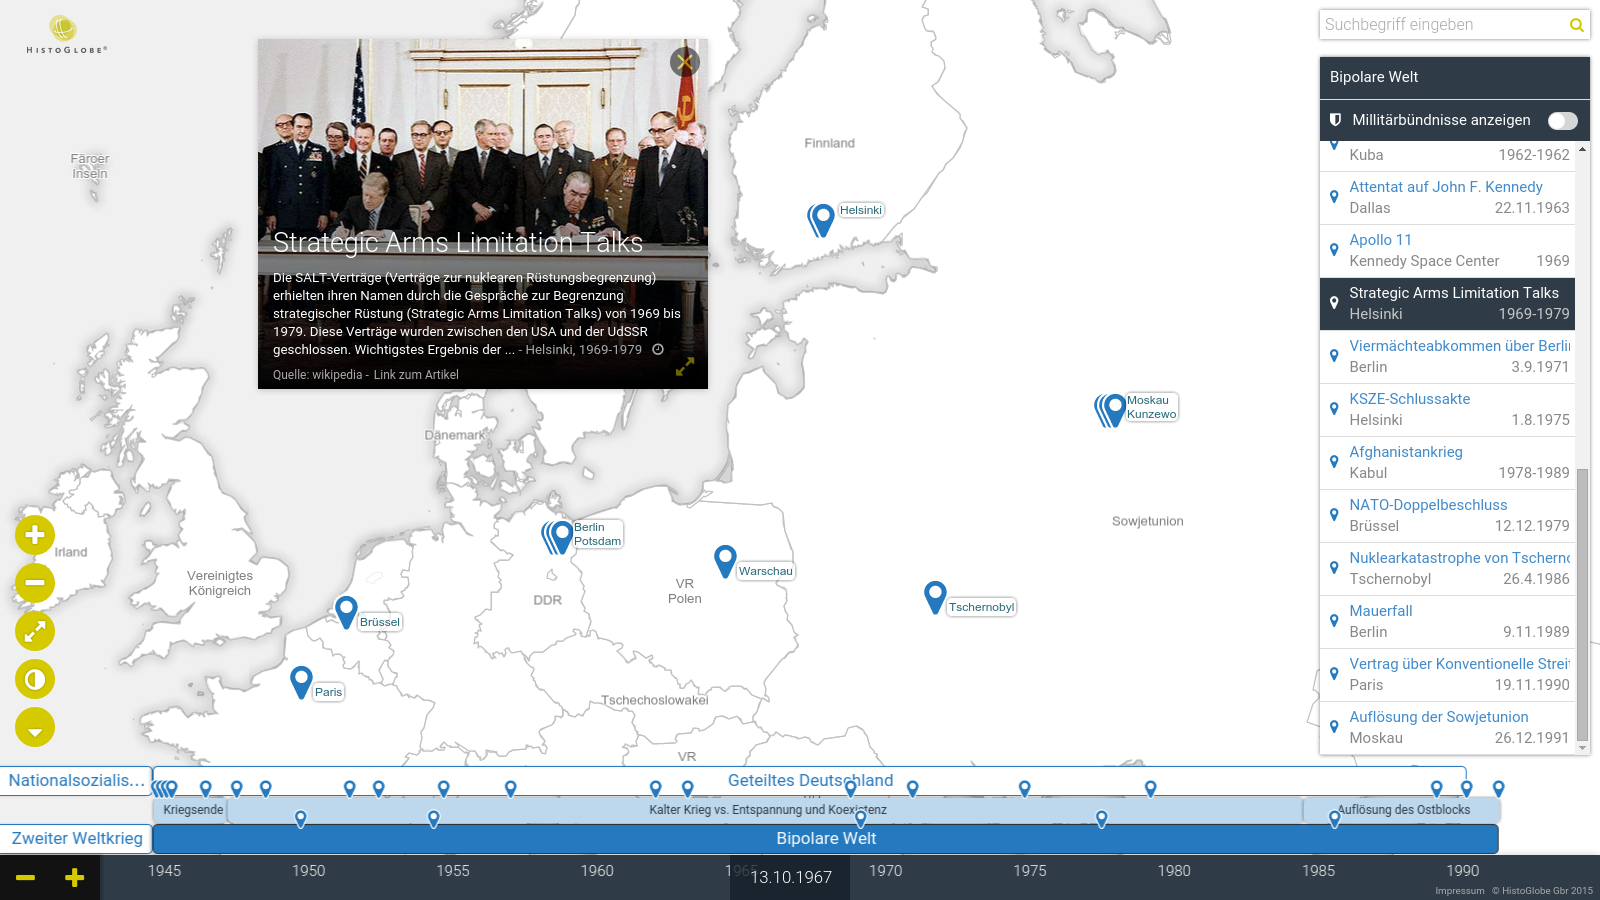
\includegraphics[width=0.9\textwidth]{graphics/final_ui.png}
  \caption{The final User Interface of \textsc{HistoGlobe}}
\end{figure}

\subsection{Map} % (fold)
\label{sub:map}

The map shows the status of the countries on Earth at this certain moment in history set in the Timeline. For this project we used a self-made dataset of historic countries of whole Europe from 1945 until today and from Western, Northern, Southern and Central Europe from 1871 until 1945. We organized the data in a way that we can visualize these historical changes of areas and names of countries. We also provided a functionality to style the country areas due to a current theme, for example all countries belonging to NATO get a blue background color.

\subsubsection{Historic Countries} % (fold)
\label{ssub:historic_countries}

A country consists of an \textbf{area}, represented as a multipolygon geometry, and a \textbf{label} with the name of the country and its position on the map.

\newpage
\paragraph{Areas}
Everything is based on a dataset of the current countries in Europe from \textit{Natural Earth Data}
\footnote{1:10m Cultural Vectors | \url{http://www.naturalearthdata.com/downloads/10m-cultural-vectors/}}.
We extracted only the countries of Europe and loaded them into \textit{QuantumGIS}, an open source GIS software for organizing, analyzing and visualizing areas on Earth. For each historic country we found an historic map online and created the area of the country using the \textit{Vector Geoprocessing Tools} of QuantumGIS. Each area is stored in a single \texttt{area\_id.geojson} file.

\begin{figure}[H]
  \begin{center}
    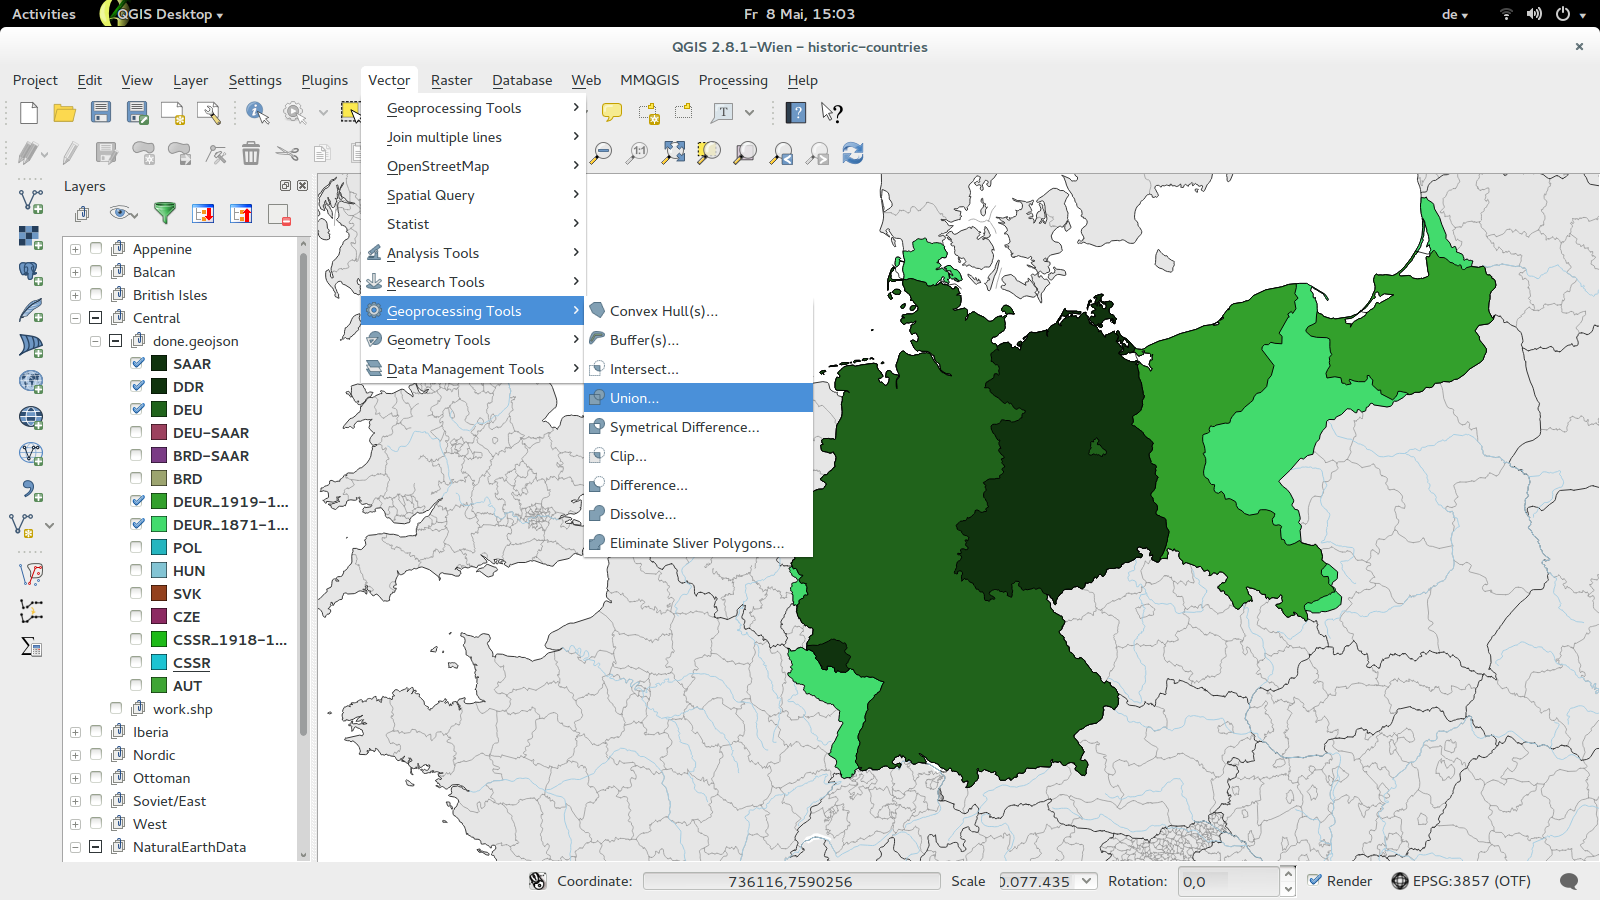
\includegraphics[width=0.9\textwidth]{graphics/qgis.png}
  \end{center}
  \caption{Geometry Manipulation of Historic Countries in QuantumGIS}
  \label{fig:qgis}
\end{figure}
\label{par:area}

\ref{fig:qgis} shows the different areas of Germany from 1871 until today, from light green to dark green:

\begin{itemize}
  \item 1871 - 1919 German Empire
  \item 1919 - 1945 Weimar Republic and Third German Reich (after WW I)
  \item 1945 - 1949 Occupied Germany (after WW II)
  \item 1949 - 1990 GDR without West Berlin and \\
        1949 - 1956 Saarland
\end{itemize}

Because of the very problematic usability of QuantumGIS and the mass of data that would have needed to be processed we have not reached the goal to create a database of all historic countries in Europe from 1871 on, due to the time constraint.

\paragraph{Labels} of a country are stored separately from the areas to account for independent changes of names and geometries: A country can be renamed and borders can change, but both events do not need to correlate. The labels are defined in a table \texttt{labels.csv} consisting of the id, the name, the position (lat, lng) and a priority.

\newpage
The visualization of the labels works with priorities. Each label has a bounding box. According to the label priority, the box increases inversely in size (low priority labels get large bounding boxes). Showing and hiding a label is based on the question if the labels collide, i.e. if their bounding boxes intersect. The algorithm works in the following way:

\begin{itemize}
  \item If a new label $L_n$ gets added to the map it checks for each shown label $L_s^H$ with a higher priority if it collides with $L_n$
  \begin{itemize}
    \item If so, $L_n$ will be hidden
    \item If it does not collide with any $L_s^H$, $L_n$ will be shown. Now it checks for each shown label with the same or lower priority $L_s^L$ if it collides with $L_n$
    \begin{itemize}
      \item If so, $L_s^L$ gets hidden
    \end{itemize}
  \end{itemize}
  \item If a label $L_r$ gets removed from the map, it checks for each hidden labels $L_h^L$ of the same and lower priority if it collides with $L_r$
  \begin{itemize}
    \item If so, $L_h^L$ gets shown
  \end{itemize}
  \item If the user zooms in, the algorithm checks for each hidden label $L_h$ if it can be shown now: it checks for each shown label $L_s^H$ of the same or higher priority if it collides with $L_h$
  \begin{itemize}
    \item If $L_h$ does not collide with any $L_s^H$, $L_h$ will be shown
  \end{itemize}
  \item If any hidden labels were toggled to be shown or if the user zooms out, the algorithm checks for each shown label $L_s$ if $L_s$ collides with any shown label of the same lower priority $L_s^L$
  \begin{itemize}
    \item If so, $L_s^L$ will be hidden
  \end{itemize}

\end{itemize}

The problem with this approach is that the label position and priority can not be deducted from the area. Therefore, both have to be set by hand. We are aware that this manual approach is not optimal, but for the scope of that project it is suitable. For the future, a data model should be found in which areas and labels are connected but can still change separately from each other.

% paragraph labels (end)

% subsubsection historic_countries (end)

\subsubsection{Historic Changes} % (fold)
\label{ssub:historic_changes}

\begin{table}[ht]
\begin{small}
  \caption{Examples of Historic Changes}
  \label{tab:changes}
  \begin{center}
    \begin{tabular}{lllllll}
    \hline

    \hline
    \textbf{date} & \textbf{name of change} & \\
    \textbf{domain} & \textbf{old} & \textbf{new} \\
    \hline
    25.12.1991 & Dissolution of Soviet Union & \\
    \textit{area:} & CCCP & \pbox{5cm}{EST, LVA, LTU, BLR, \\ UKR, MDA, RUS} \\
    \textit{label:} & CCCP & \pbox{5cm}{EST, LVA, LTU, BLR, \\ UKR, MDA, RUS }\\
    \hline
    03.10.1990 & German reunification & \\
    \textit{area:} & BRD, DDR & DEU \\
    \textit{label:} & BRD, DDR & DEU \\
    \hline
    01.01.1990 & End of Socialistic Republics & \\
    \textit{area:} & -- & -- \\
    \textit{label:} & PR-ROU, PR-BGR, PR-HUN, PR-POL & ROU, BGR, HUN, POL \\
    \hline
    01.01.1979 & Separation of Greenland & \\
    \textit{area:} & DNK-with-GRL & DNK, GRL \\
    \textit{label:} & -- & GRL \\
    \hline
    01.01.1881 & Init state & \\
    \textit{area:} & -- & DEU-REICH-1871, POL-1871, ... \\
    \textit{label:} & -- & DEU-REICH-1871, POL-1871, ... \\
    \hline

    \hline
    \end{tabular}
  \end{center}
\end{small}
\end{table}

Because of the way areas and labels are organized, an historic change can easily be modeled, like seen in \ref{tab:changes}. This event-based data model is maintained like this: if an historic change happens, it needs to have a date and a name of the change, a set of areas that stop exist and a set of areas that start to exist from this date in history on -- the same for the labels. Afterwards, the new areas have to be created in \textit{QuantumGIS}, which is most of the work, and new labels have to be defined in the table.

In order to visualize the data on the client side, the areas, labels and changes have to be preprocessed on the server. Especially the transition areas and borders have to be generated.

\newpage
\paragraph{Transitions} are the geometric changes in a change event. There is either a transition area, which is the area that changes the membership of a country (e.g. Alsace-Lorraine 1919 from the German Empire to France) or a transition border, that splits two countries (e.g. The border between Czech and Slovak Republic after the dissolution of Czechoslowakia in 1991). These transitions shall be emphasized with an animation in the moment of the historic change so that it is clearly visible to the user what is currently happening. The transitions are generated like this: For each historic change the set of old and new areas are compared to each other and pass the following decision tree:

% Set the overall layout of the tree
\tikzstyle{level 1}=[level distance=1.5cm, sibling distance=6.5cm]
\tikzstyle{level 2}=[level distance=2cm, sibling distance=2.8cm]
\tikzstyle{level 3}=[level distance=2.5cm, sibling distance=2.8cm]

% Define styles for bags and leafs
\tikzstyle{bag} = [text width=3.5cm, text centered]

% The sloped option gives rotated edge labels. Personally
% I find sloped labels a bit difficult to read. Remove the sloped options
% to get horizontal labels.
\begin{center}
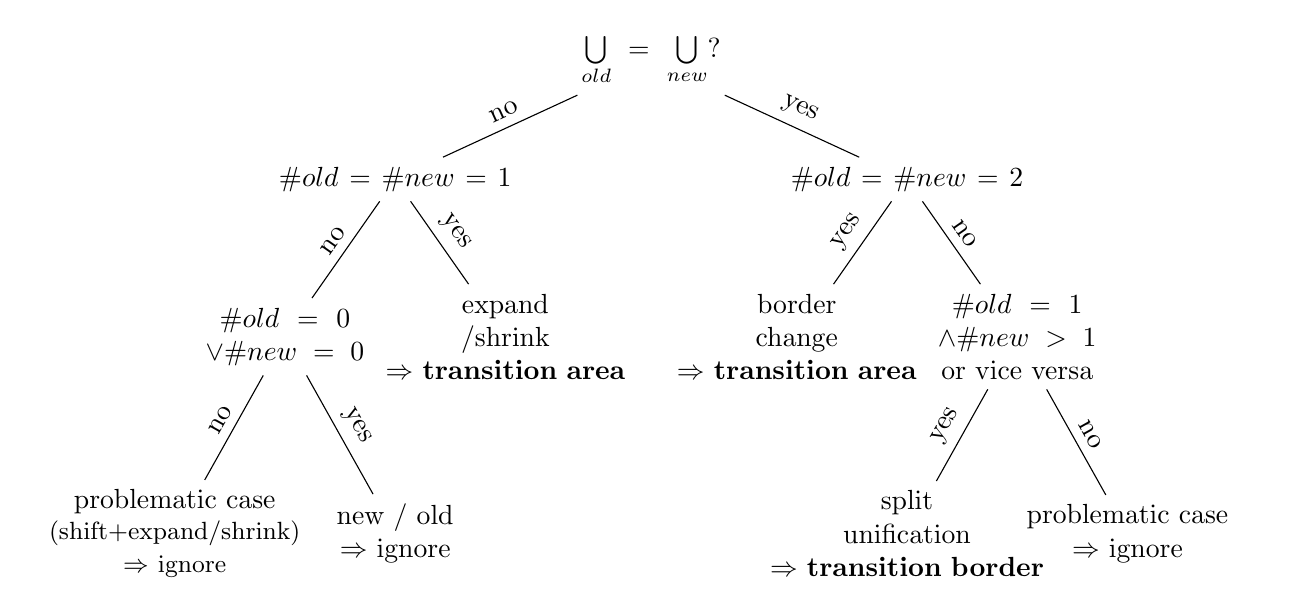
\begin{tikzpicture}[grow=down, sloped]
\node[bag] {$\bigcup\limits_{old}=\bigcup\limits_{new} ?$}
  child
  {
    node[bag] {$\#old=\#new=1$}
    child
    {
      node[bag] {$\#old=0$ \\ $\vee \#new=0$}
      child
      {
        node[bag] {problematic case \\ \small{(shift+expand/shrink)} \\ $\Rightarrow$ ignore}
        edge from parent
        node[above] {no}
      }
      child
      {
        node[bag] {new / old\\ $\Rightarrow$ ignore}
        edge from parent
        node[above] {yes}
      }
      edge from parent
      node[above] {no}
    }
    child
    {
      node[bag] {expand\\/shrink \\ $\Rightarrow$ \textbf{transition area}}
      edge from parent
      node[above] {yes}
    }
    edge from parent
    node[above] {no}
  }
  child
  {
    node[bag] {$\#old=\#new=2$}
    child
    {
      node[bag] {border\\change \\ $\Rightarrow$ \textbf{transition area}}
      edge from parent
      node[above] {yes}
    }
    child
    {
      node[bag] {$\#old=1$ \\ $\wedge \#new>1$ \\ or vice versa}
      child
      {
        node[bag] {split\\unification \\ $\Rightarrow$ \textbf{transition border}}
        edge from parent
        node[above] {yes}
      }
      child
      {
        node[bag] {problematic case \\ $\Rightarrow$ ignore}
        edge from parent
        node[above] {no}
      }
      edge from parent
      node[above] {no}
    }
    edge from parent
    node[above] {yes}
  };
\end{tikzpicture}
\end{center}

\begin{center}
\begin{small}
  \textit{Legend:} $old$ = set of all old areas, $new$ = set of all new areas \\
  $\bigcup\limits_{old}$ = union of all old areas, $\#old$ = number of old areas
\end{small}
\end{center}

\vspace{0.5cm}

\paragraph{Preprocessing} happens with a \textit{Python} script performing the following steps:

\begin{enumerate}
  \item Loading the areas (from \textit{*.geojson}), the labels and the changes (from \textit{*.csv})
  \item Checking the set of areas and labels for completeness and the changes for consistency
  \item Generating the transition areas
  \item Writing the data to \textit{json} files to be delivered to the client:
  \begin{enumerate}
    \item \texttt{areas.geojson}
    \item \texttt{labels.geojson}
    \item \texttt{trans\_areas.geojson}
    \item \texttt{changes.json}
  \end{enumerate}
\end{enumerate}

\paragraph{The Workflow}
at runtime of the program can be seen in \ref{fig:historic_changes}. The diagram is simplified focusing only on the areas, but the process is the same for the labels.

\begin{figure}[H]
  \begin{center}
    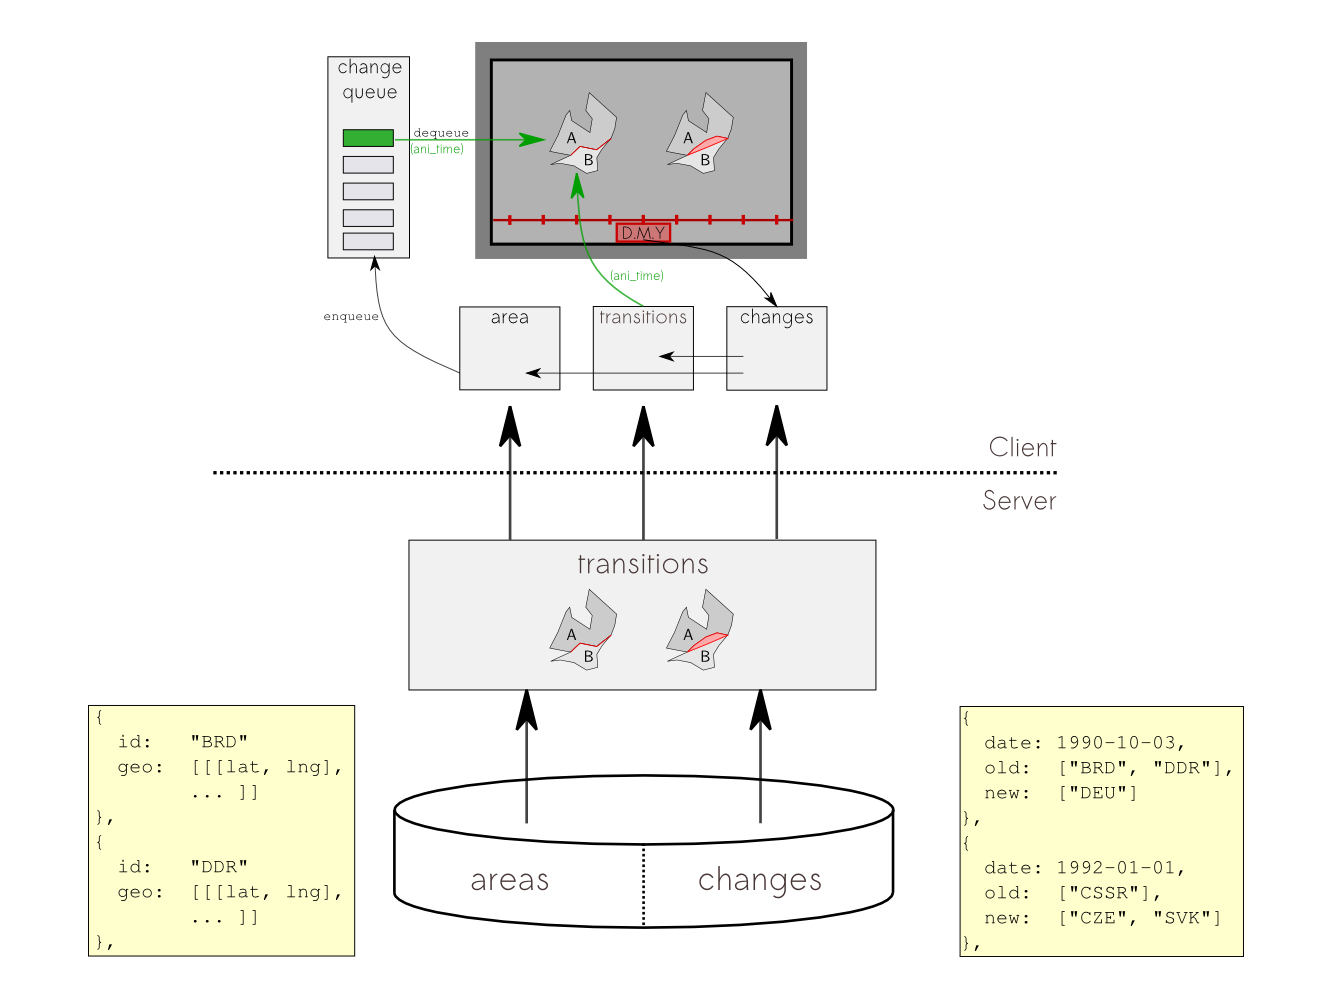
\includegraphics[width=0.9\textwidth]{graphics/historic_countries.png}
  \end{center}
  \caption{Architecture of historic countries on the map}
  \label{fig:historic_changes}
\end{figure}

The countries areas, labels and changes are created, preprocessed and loaded to the server. The client gets the four \textit{json} files and reads the data out of them. If the NowDate changes, the Timeline sends the old date and the new date to the Controller that finds out all the changes happened in that time period. For each change the transition areas and borders are faded in on the map and the related old and new areas and labels are enqueued as a change event in a \textbf{change queue}. Every 50 milliseconds the queue is processed: for the first change event it checks if the related transitions are fully faded in. If so, the new areas and labels will be added and the old areas and labels deleted from the map. Finally, the transitions will be faded out again. This is repeated until the first change in the queue is not ready to be executed.

For moving the Timeline backwards the mechanism is the same, it is just that old and new areas and labels are swapped, because the historic change happens the other way.

In order to prevent large amounts of changes on the map if the Timeline is moved far, a rule-out mechanism is implemented: There is a list of old and new areas and labels for all historic changes in the period between the old and the new date from the Timeline. Areas and labels that would be added in one change but deleted in another one are removed from both lists, because they would not contribute to the current state. With this mechanism it is possible to move the Timeline at a high speed there and back and always get a fast and consistent update on the map.


\subsubsection{Styling the Countries} % (fold)
\label{ssub:styling_the_countries}

Each area and each label can have a certain style in a certain \textbf{theme}. An example theme we have implemented is called \textit{Bipolar World} (Figure \ref{fig:biplar_world}) and assigns each country in Europe a membership to the NATO (blue) and the Warsaw Pact (red) based on their dates of joining and leaving the alliance. When moving the timeline the user can see how the alliances develop.

\begin{figure}[H]
  \begin{center}
    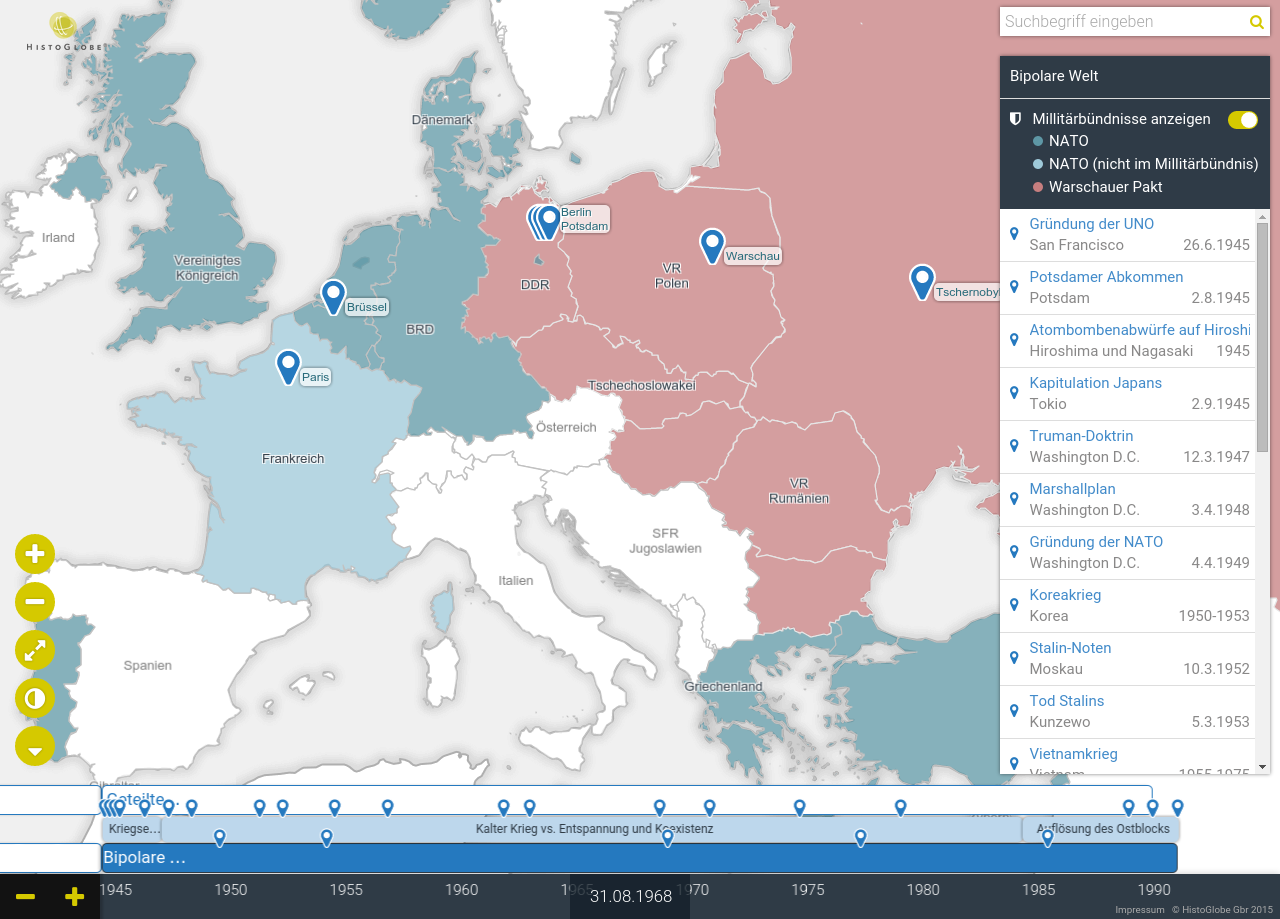
\includegraphics[width=0.9\textwidth]{graphics/bipolar_world.png}
  \end{center}
  \caption{Countries colored due to their membership in NATO or Warsaw Pact}
  \label{fig:biplar_world}
\end{figure}

The style module was designed in a reusable way: for any new theme there have to be firstly \textbf{class}es and their styles defined (e.g. \texttt{class: nato}, ~\texttt{background-color: blue}). Secondly, areas and the membership to a class have to be stated in a table with \texttt{area\_id}, \texttt{theme\_class}, \texttt{start\_date}, \texttt{end\_date} (e.g. \texttt{ESP, NATO, 1982, 1986}). The same has to be done with labels.


% subsubsection styling_the_countries (end)

% subsection map (end)

\section{Timeline and Topic Bars}
Timeline von Mädelsmentor
\subsection{Search Bar} % (fold)
\label{sub:search_bar}

One way to retrieve information about historical events is our search bar, which is a single-line text box with the dedicated function of accepting user input to be searched for. The user is able to search for events, people, places and time.

\begin{figure}[H]
  \begin{center}
    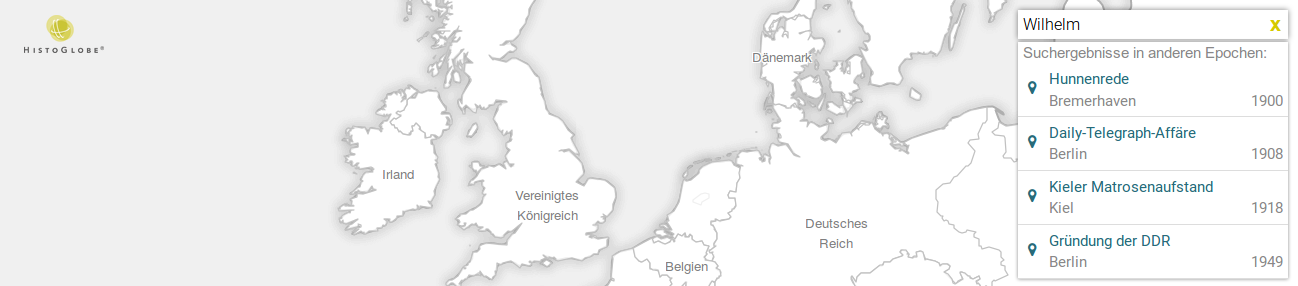
\includegraphics[width=0.9\textwidth]{graphics/search.png}
  \end{center}
  \caption{Search Bar with some search results in drop-down list}
  \label{fig:search}
\end{figure}
%\label{par:search}

\paragraph{Search Algorithm}
\label{par:search_alg}
The search algorithm uses the underlying data structure to improve the search process. Each Hivent has a title, location, time and e description. We search over all Hivents and if we match we are looking for the next. So each Hivent appears only once in out result list. Out algorithm has a special search structure. At first we are looking in the tile, location and tine data field. Than we are looking in the description of the Hivents and parse for text snippets. All results are sorted in search results of the current epoch and search results of other epochs.
% paragraph search algorithm (end)

\paragraph{Instant Search} % (fold)
\label{par:instant_search}
All possible matches are immediately displayed while the user is typing text. So the search is sent automatically to present the user with real-time results which are displayed as a drop-down list. This often allows the user to stop short of typing the entire word they were looking for.
% paragraph instant search (end)

% subsection search_bar (end)

\section{Hivent List}
Platzhalter\\
\newpage
\subsection{Hivent Boxes}
In HistoGlobe Hivent Boxes are the main method to display information beside the name, the location or the date of an historical event (Hivent). Every Hivent Box consists of a name, a short description about the Hivent, a link to the article on Wikipedia and multimedia content like an image or a video, if such a thing exists for the Hivent.

\begin{figure}[H]
  \begin{center}
    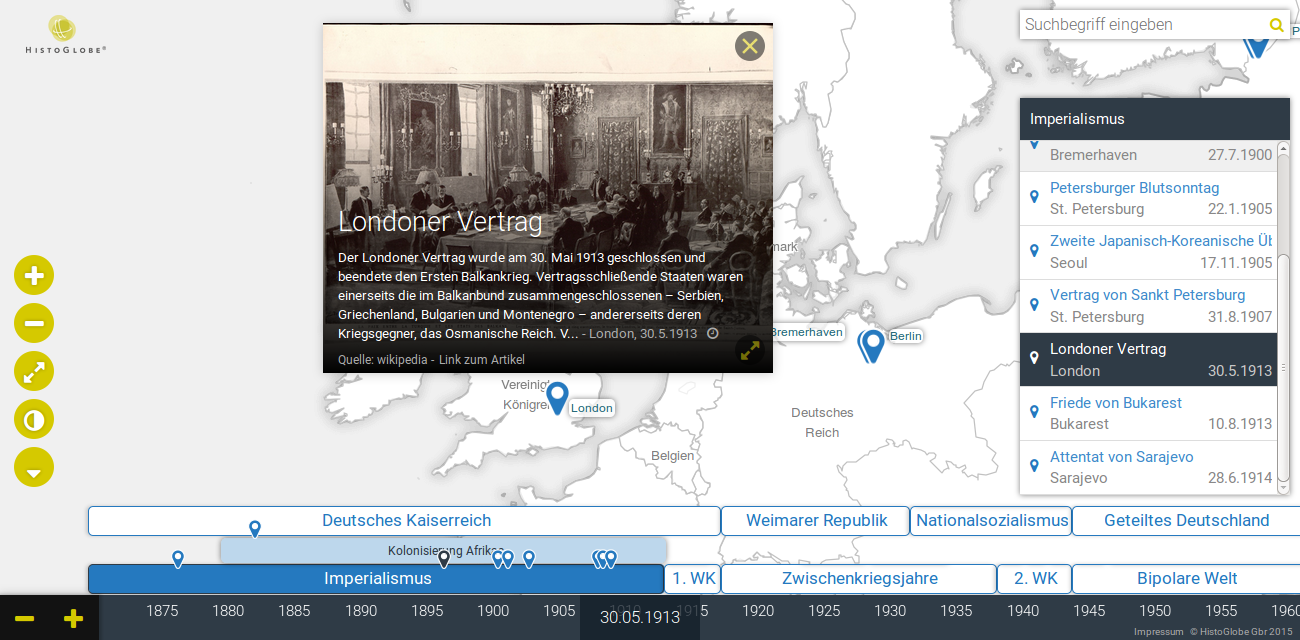
\includegraphics[width=0.9\textwidth]{graphics/hivent_box.png}
  \end{center}
  \caption{Hivent Box displaying information of an historical event with an image}
  \label{fig:hivent_box}
\end{figure}


\paragraph{Small Hivent Box} % (fold)
The small version, as displayed in figure \ref{fig:hivent_box}, is the default representation of our Hivent Boxes. This version is moveable on the map per drag and drop and consists of the same information like the the big Hivent Box, but with a smaller description length.

\paragraph{Big Hivent Box} % (fold)
In figure \ref{fig:hivent_box_big} you can see the big Hivent Box. As mentioned above this version differs only in description length from the small Hivent Box and of course in its size. 

\begin{figure}[H]
  \begin{center}
    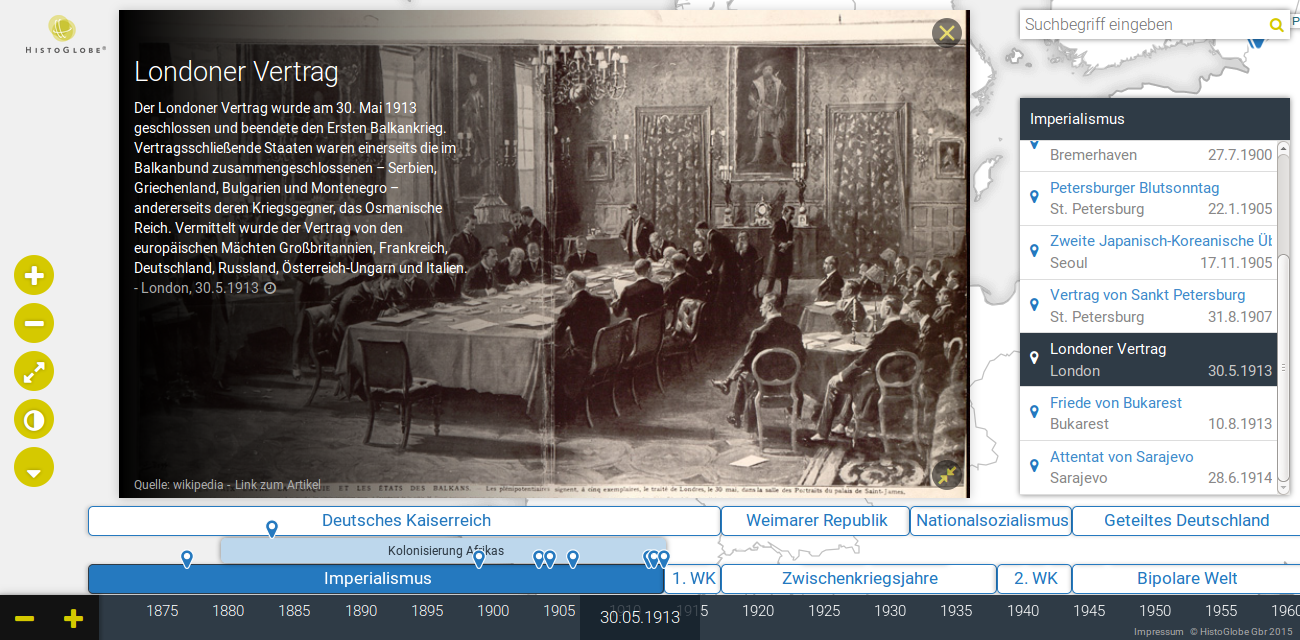
\includegraphics[width=0.9\textwidth]{graphics/hivent_box_big.png}
  \end{center}
  \caption{Big Hivent Box}
  \label{fig:hivent_box_big}
\end{figure}
\label{par:hivent_box_big}

\paragraph{Resize Button - Extend} % (fold)
This button downright is only available in the small version of the Hivent Box and allows the user to switch to the big Hivent Box. 
\paragraph{Resize Button - Compress} % (fold)
This button downright is only available in the big version of the Hivent Box and allows the user to switch back to the small Hivent Box.
\paragraph{Multimedia Button} % (fold)
This button on the right is available in both versions of the Hivent Box, the small and the big one, but only if there is existing multimedia content. With this button the user can switch to the multimedia content.

\begin{figure}[H]
  \centering
  \begin{minipage}{0.49\textwidth}
    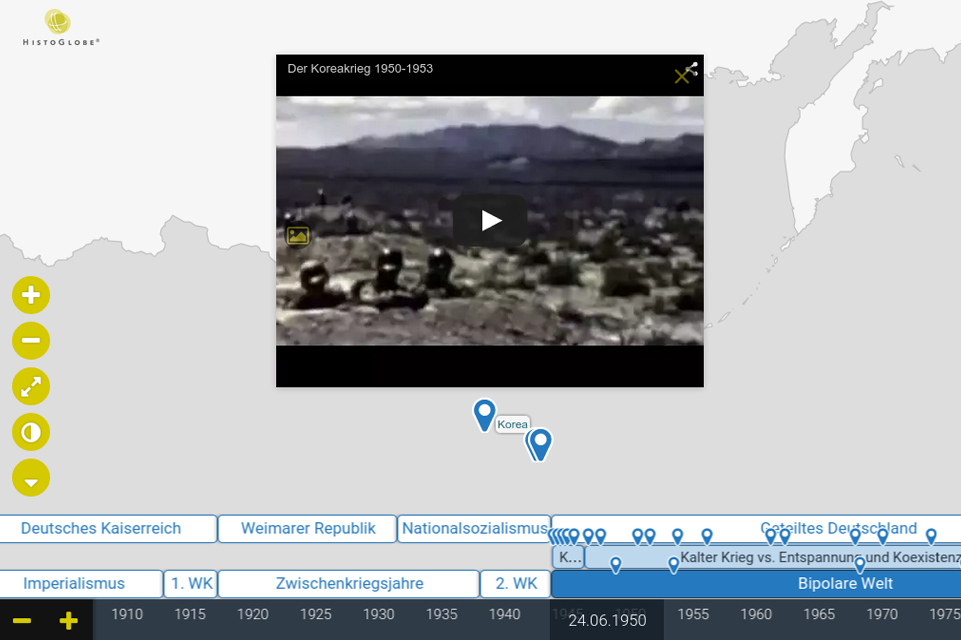
\includegraphics[width=0.95\textwidth]{graphics/smallBox_MM.png}
  \end{minipage}
  \label{fig:multimedia_content_small}
  \begin{minipage}{0.49\textwidth}
    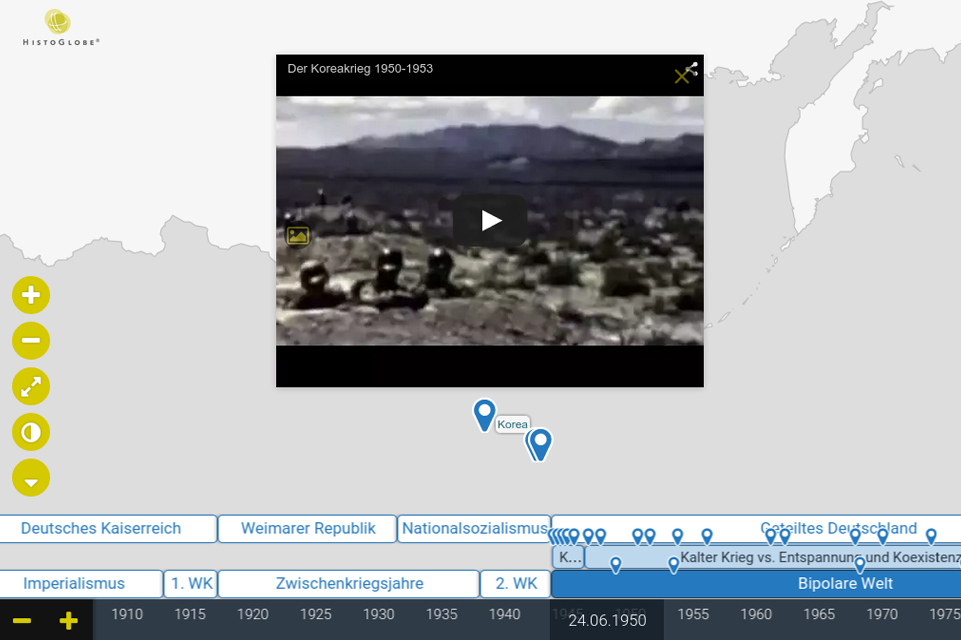
\includegraphics[width=0.95\textwidth]{graphics/bigBox_MM.png}
  \end{minipage}
  \caption{Multimedia content in small and big Hivent Box}
  \label{fig:multimedia_content_small}
\end{figure}
\label{par:multimedia_button}

\paragraph{Image Button} % (fold)
This button on the left is only available in the multimedia view of the Hivent Box and allows the user to switch back to normal view. 
\paragraph{Close Button} % (fold)
This button in the right upper corner is available in every view and version of the Hivent Box and allows the user to close the box.
\subsection{Control Buttons} % (fold)
\label{sub:control_buttons}
\begin{minipage}{0.05\textwidth}
	
\includegraphics[width=0.95\textwidth]{graphics/plus.png}
\end{minipage}
\label{fig:controll_button_plus}
~
\begin{minipage}{0.94\textwidth}
	Change the size of the map - zoom in\\
\end{minipage}
~
\begin{minipage}{0.05\textwidth}
	
\includegraphics[width=0.95\textwidth]{graphics/minus.png}
\end{minipage}
\label{fig:controll_button_minus}
~
\begin{minipage}{0.94\textwidth}
	Change the size of the map - zoom out\\
\end{minipage}
~
\begin{minipage}{0.05\textwidth}
	
\includegraphics[width=0.95\textwidth]{graphics/resize.png}
\end{minipage}
\label{fig:controll_button_resize}
~
\begin{minipage}{0.94\textwidth}
	Switch to fullscreen mode or back to normal view if fullscreen mode is active\\
\end{minipage}
~
\begin{minipage}{0.05\textwidth}
	
\includegraphics[width=0.95\textwidth]{graphics/HC.png}
\end{minipage}
\label{fig:controll_button_HC}
~
\begin{minipage}{0.94\textwidth}
	Enable high contrast mode or switch back to normal view if high contrast mode is active\\
\end{minipage}
~
\begin{minipage}{0.05\textwidth}
	
\includegraphics[width=0.95\textwidth]{graphics/minUi.png}
\end{minipage}
\label{fig:controll_button_HC}
~
\begin{minipage}{0.94\textwidth}
	Minimal user interface - hide/show Hivent List and Topic Bars
\end{minipage}
~
% subsection control_buttons (end)

\subsection{Hivents} % (fold)
\label{sec:hivents}

Hivents mean ``Historical Events''. They are the way historical events are defined and presented. They are stored in a database, and have attributes such as name, location, start- and endyear, description and associated media.
They are one of the most important concepts to visualize history in HistoGlobe.

% subsection general (end)
\subsubsection{Behavior} % (fold)
\label{sub:behaviour}
Hivents are represented on several locations in the UI, with the map, the Hivent-List and the Timeline being the most important ones.
Since usually more than one Hivent is being shown, it's important to signify the representation between one Hivent in different UI-Elements.
The main interface events to which the feedback occurs are mouse hovering and clicking, which leads to the Hivent being highlighted in all UI-elements.

\begin{figure}[ht]
  \begin{center}
    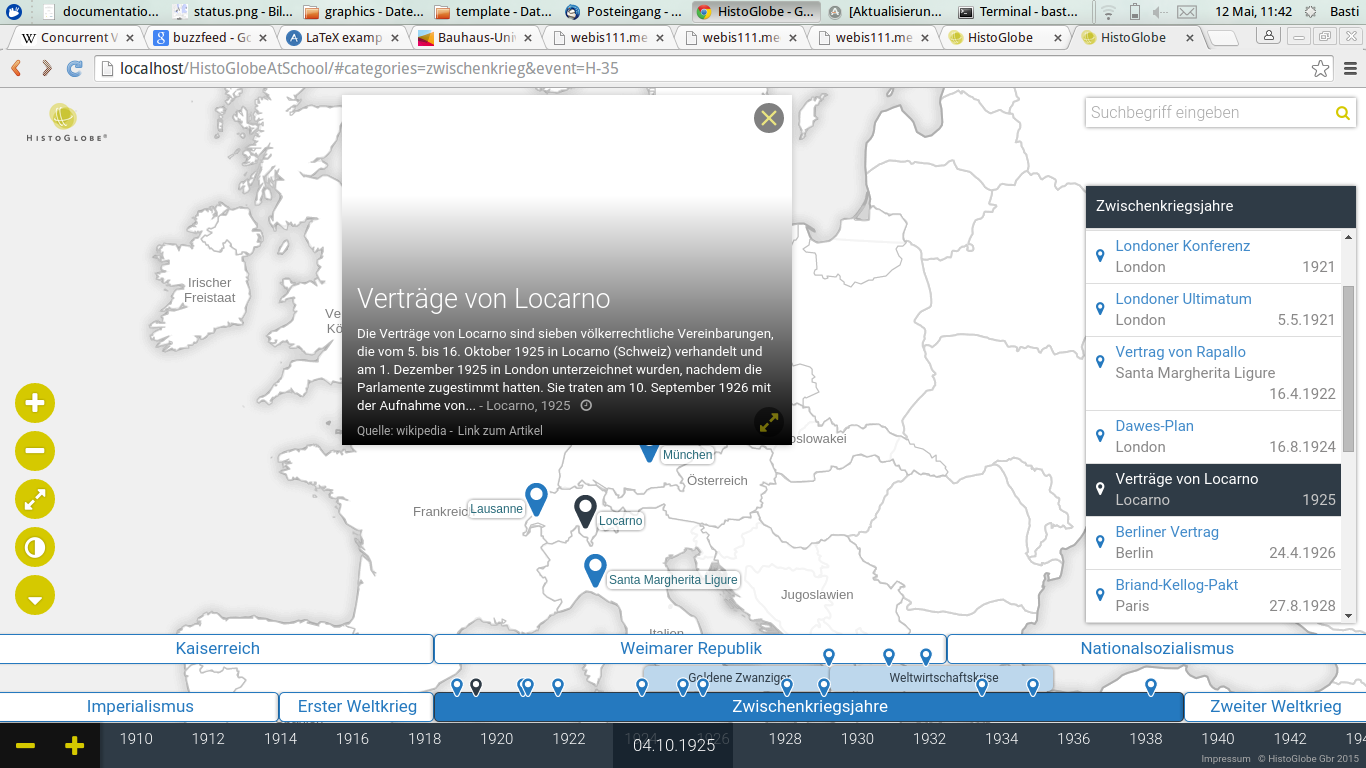
\includegraphics[width=0.8\textwidth]{graphics/activated_hivent.png}
  \end{center}
  \caption{Activated Hivent}
  \label{fig:activated_hivent}
\end{figure}

Upon being clicked on, it changes its status to active. An active Hivent gets focused in the map, it's marker are highlighted, it gets tagged in the URL bar and the Hivent box opens.

\subsubsection{Labels on Map}
Hivents on the Map were only represented by a marker.
Upon being very close they get automatically clustered.

The teacher demanded more information, so we attached labels to the Hivent markers.
We tried a Leaflet addon, but it didn't match our expectations of modifiability.
To do labels our own, we used how the markers were implemented in the first space. They are Leaflet DivIcons so they are a div with a background image essentially. To accomplish easily modifiable labels we simply added another div element.

In the first implementation the Hivents name was shown, but we realized this isn't appropriate on a map, so we switched to show the Hivents location. With this solution we got easily modifiable small weight labels.

To adjust them to reasonable readability we had to fulfill special requirements.
We needed an algorithm which was  particularly lightweight, since we can't precompute the labels positioning and due to the fact that we wanted to use \HG on school pcs and mobile devices.
Our solution is done by checking for an overlap by comparing the divs Bounding Boxes and moving the left label to the left on overlap.

On high zoom levels the amount of labels was so high the map wasn't readable anymore, so we remove them from a certain zoom level on.

  \begin{figure}[H]
\begin{center}
  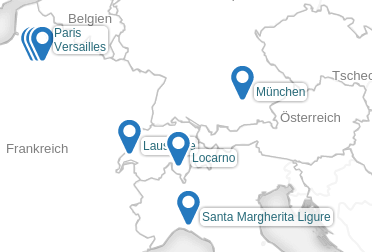
\includegraphics[width=0.4\textwidth]{graphics/overlapping_labels_2.png}
  \end{center}

  \caption{Overlapping labels}
  \label{fig:overlapping_labels}
  \end{figure}

\subsubsection{Hivent Regions}
A lot of historical events took place over a region, such as wars, so we wanted a region representation of hivents on the map.
We implemented an additional type of map marker to do this.
We added an additional optional attribute to the hivents, containing the polygon representing the region.
The implementation was done using Leaflets Polygon drawing capabilites.

  \begin{figure}[H]
\begin{center}
  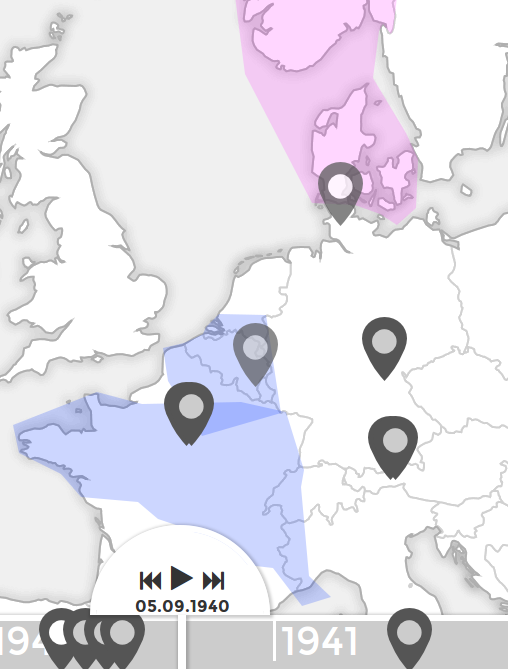
\includegraphics[width=0.3\textwidth]{graphics/status2.png}
  \end{center}

  \caption{Hivent regions with highlights}
  \label{fig:hivent_region_highlight}
  \end{figure}

% subsection hghghg (end)
% section section_name (end)

% subsection behaviour (end)
% section hivents (end)


% section user_interface_elements (end)
